\documentclass[]{article}
\usepackage{amsmath,amssymb,amsthm}
\usepackage[utf8]{inputenc}
\usepackage{lmodern}
%\usepackage{circuitikz}
\makeatletter
\@ifpackageloaded{tex4ht}{
    \def\pgfsysdriver{pgfsys-tex4ht.def}
}
\makeatother
\usepackage{pgfplots}
\usepackage{pgfplotstable}
\usepackage{pgf,tikz}
\usetikzlibrary{shapes,backgrounds,positioning,matrix,decorations}

\usepackage{siunitx}
\usepackage{python}
\usepackage{ifxetex,ifluatex}
\usepackage{listings}
\setlength{\parskip}{3mm}
\newtheorem{axiom}{Axiom}
\newtheorem{definition}{Definition}
\newtheorem{comment}{Comment}
\newtheorem{example}{Example}
\newtheorem{lemma}{Lemma}
\newtheorem{property}{Property}
\newtheorem{problem}{Problem}
\newtheorem{remark}{Remark}
\newtheorem{theorem}{Theorem}
\newtheorem{script}{Script}

\usepackage{fixltx2e} % provides \textsubscript
% use upquote if available, for straight quotes in verbatim environments
\IfFileExists{upquote.sty}{\usepackage{upquote}}{}
\ifnum 0\ifxetex 1\fi\ifluatex 1\fi=0 % if pdftex
  \usepackage[utf8]{inputenc}
\else % if luatex or xelatex
  \ifxetex
    \usepackage{mathspec}
    \usepackage{xltxtra,xunicode}
  \else
    \usepackage{fontspec}
  \fi
  \defaultfontfeatures{Mapping=tex-text,Scale=MatchLowercase}
  \newcommand{\euro}{€}
\fi
% use microtype if available
\IfFileExists{microtype.sty}{\usepackage{microtype}}{}
\usepackage{graphicx}
% Redefine \includegraphics so that, unless explicit options are
% given, the image width will not exceed the width of the page.
% Images get their normal width if they fit onto the page, but
% are scaled down if they would overflow the margins.
\makeatletter
\def\ScaleIfNeeded{%
  \ifdim\Gin@nat@width>\linewidth
    \linewidth
  \else
    \Gin@nat@width
  \fi
}
\makeatother
\let\Oldincludegraphics\includegraphics
{%
 \catcode`\@=11\relax%
 \gdef\includegraphics{\@ifnextchar[{\Oldincludegraphics}{\Oldincludegraphics[width=\ScaleIfNeeded]}}%
}%
\ifxetex
  \usepackage[setpagesize=false, % page size defined by xetex
              unicode=false, % unicode breaks when used with xetex
              xetex]{hyperref}
\else
  \usepackage[unicode=true]{hyperref}
\fi
\hypersetup{breaklinks=true,
            bookmarks=true,
            pdfauthor={Dilawar Singh},
            pdftitle={Assignment - Lecture 06},
            colorlinks=true,
            citecolor=blue,
            urlcolor=blue,
            linkcolor=magenta,
            pdfborder={0 0 0}}
\urlstyle{same}  % don't use monospace font for urls
\setlength{\parindent}{0pt}
\setlength{\parskip}{6pt plus 2pt minus 1pt}
\setlength{\emergencystretch}{3em}  % prevent overfull lines
\setcounter{secnumdepth}{0}

\title{Assignment - Lecture 06}
\author{Dilawar Singh}
\date{}

\begin{document}
\maketitle

\textbf{1. Exorcism Maxwell's Demon}

\begin{quote}
``Concerning Demons: 1. Who gave them this name? Thomson'' -- In a
letter from Maxwell to Tait
\end{quote}

Unless demon does some work to create the heat-gradient in given system,
the second law of thermodynamics -- a heat engine with efficiency more
than 1 -- is violated. The demon is exorciated by showing that this is
not the case and Demon has to do some work to create such a temperature
gradient; even when closing and opening of gate does not involve any
work.

\textbf{Given that Demon is governed by laws of thermodynamics itself},
an information theoretic approach is wildely believed to exorcise
Maxwell's Demon. The thesis was first proposed by Slizard where he
asserts, 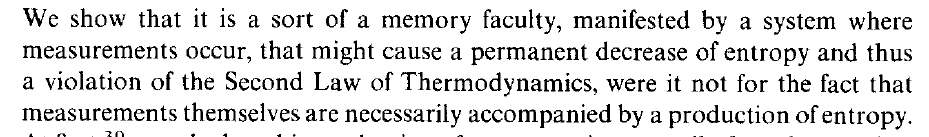
\includegraphics{./slizard.png}

Moreover, Slizard project which establishes that there is a cost to
information actuition is meant to protect the 2nd law not from the
fluctuation phenomenon, but only from the intelligent accumulation of
fluctuations.

Assume that we have 6 buckets in which we are to put 20 balls. In first
case, we put 20 balls in 3 buckets; other 3 buckets are empty. The
entropy of this system is $A \times ln \frac{20!}{n_1! n_2! n_3!}$. If
Demon partitions the balls into two sets of 10 balls each without doing
any work, then the entropy of new system is
$A \times ln \frac{10!}{n_1! n_2! n_3!} + A \times \frac{10!}{n_1! n_2! n_3!}$,
where $n_1$, $n_2$, and $n_3$ are values from a distribution but with
the contrains that $n_1 + n_2 + n_3 = 10$ or 20 depending on the
context.

Then exorcising the Demon is as simple as showing that entropy in the
second case is lower than the first case. Therfore Demon must have done
some work to lower the entropy the system.

\textbf{2. Plot $\frac{N_2}{N_1}$ for a two state system as a function
of temperature (2 - 5000 $K$) for $\delta E = 0.05, 0.5, 1$, and
\SI{5}{kcal/mole}.}

If the number of molecules in state $i$ is $N_i$, and number of
molecules in the ground-most state are $N_0$; and if
$\Delta E = E_i - E_0$ then we have the following relationship:

\[ N_i = N_0 \exp{ \frac{-\Delta E}{k_B T}} \]

This equation is reduced to the following once we put the values of
constants in dimensions given in assignment.

\[ \frac{N_i}{N_0} = \exp{\frac{- \Delta E}{1.987\times 10^{-3}T}} \]

Now we can plot the function. Plot is shown in figure \ref{fig:1}.

\begin{figure}[h!]
\label{fig:1}
\begin{tikzpicture}[scale=1]
    \begin{axis} [ xlabel={Temperature in Calvin}
            , ylabel = {$\frac{N_i}{N_0}$}
            , legend style={legend pos=outer north east}
        ]
        \foreach \e in {0.05, 0.5,1,5} {
            \addplot+[smooth,domain=2:5000]{exp(-\e/(1.987e-3 * x)};
            \addlegendentryexpanded{\e};
        };
    \end{axis}
\end{tikzpicture}
\caption{$T$ and distribution for various $\Delta E$ values.}
\end{figure}

\textbf{3. Plot of $\frac{N_i}{N_0}$ vs $\Delta E$}

This plot is in figure \ref{fig:2}.

\begin{figure}[h!]
\label{fig:2}
%% Another figure
\begin{tikzpicture}[scale=1]
    \begin{axis} [ xlabel={$\Delta E$}
            , ylabel = {$\frac{N_i}{N_0}$}
            , legend style={legend pos=outer north east}
        ]
        \foreach \t in {5,50,100,500,1000,5000} {
            \addplot+[smooth,domain=0.1:5]{exp(-x/(1.987e-3 * \t)};
            \addlegendentryexpanded{\t};
        };
    \end{axis}
\end{tikzpicture}
\caption{$\Delta E$ and distribution for various temperatures}
\end{figure}

\textbf{4. Sun Vs Human}

The mass of Sun is estimated to be $1.989e30$ Kg and total power of Sun
is $3.95e26$ Watt. Therefore, power of Sun per unit mass is 1.986e-4
Watt per Kg. In 2008, it was estimated that we use 142.3 kWh per capita
i.e.~39.53 W per capita. The average weight of human is 62 Kg. Therefore
energy consumption per unit mass by a human is approximately 0.64 W per
Kg.

The ratio of power produced by sun per unit mass to the ratio of power
consumed by human per unit mass is 0.003255.

\end{document}
